\section{Materiais e Métodos}

\subsection{Descrição do problema}
O capítulo \ref{chap2} apresentou o desenvolvimento de um código em LUA.

\subsection{Funções}

\subsubsection*{draw\_square()}
\begin{itemize}
  \item Nome da função: \textbf{draw\_square}.
  \item Descrição: Desenha um quadrado a partir do vetor de pontos do argumento da função.
  \item Argumentos de entrada: Vetor \textbf{points}.
  \item Retorno: vazio.
\end{itemize}

\subsubsection*{draw\_circle()}
\begin{itemize}
  \item Nome da função: \textbf{draw\_circle}.
  \item Descrição: Desenha um círculo a partir do vetor de pontos do argumento da função.
  \item Argumentos de entrada: Vetor \textbf{points}.
  \item Retorno: vazio.
\end{itemize}

\subsection*{do\_draw()}
\begin{itemize}
  \item Nome da função: \textbf{do\_draw}
  \item Descrição: Realiza a construção geométrica do problema estudado (circuito magnético, enrolamentos, região de contorno)
  \item Argumentos de entrada: vazio.
  \item Retorno: vazio.
\end{itemize}

\subsection*{do\_materials()}
\begin{itemize}
  \item Nome da função: \textbf{do\_materials}
  \item Descrição: Define os materiais a serem utilizados no problema (\textit{Ar}, \textit{30 AWG} e \textit{US Steel Type 2-S 0.018 inch thickness})
  \item Argumentos de entrada: vazio.
  \item Retorno: vazio.
\end{itemize}

\subsection*{do\_circuit()}
\begin{itemize}
  \item Nome da função: \textbf{do\_circuit}
  \item Descrição: Define o circuito elétrico nos enrolamentos do material magnético (Ic+ = 0.1[A] e Ic- = -0.1[A]).
  \item Argumentos de entrada: vazio.
  \item Retorno: vazio.
\end{itemize}

\subsection*{do\_blocks()}
\begin{itemize}
  \item Nome da função: \textbf{do\_blocks}
  \item Descrição: Define os blocos da figura e define os tipos de materiais em cada bloco.
  \item Argumentos de entrada: vazio.
  \item Retorno: vazio.
\end{itemize}

\subsection*{do\_mesh()}
\begin{itemize}
  \item Nome da função: \textbf{do\_mesh}
  \item Descrição: Realiza o processo de triangulação
  \item Argumentos de entrada: vazio.
  \item Retorno: vazio.
\end{itemize}

\subsection*{do\_plots()}
\begin{itemize}
  \item Nome da função: \textbf{do\_plots}
  \item Descrição: Realiza a construção e exibição dos gráficos (densidade de fluxo magnético, potencial elétrico, intensidade de campo)
  \item Argumentos de entrada: vazio.
  \item Retorno: vazio.
\end{itemize}

\subsection{Arquivos}
\begin{figure}[H]
\centering
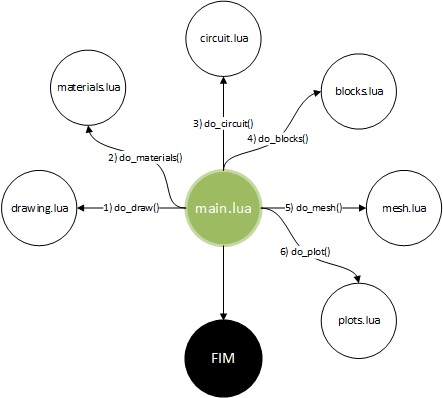
\includegraphics[scale=1]{img/assig3/main_program_subprograms.png}
\caption[Resultados]{Funções de cada subprograma acessadas pelo programa main.tex}
\label{lua_mesh}
\end{figure}
